\section{Neuronale Netzwerke}\label{sec:10-neuronale-netzwerke}

\begin{contentbox}
Neuronale Netzwerke (Neural Networks, NNs) bestehen aus vielen kleinen Funktionseinheiten, den sogenannten \ZSFkeyword*{Neuronen}. Diese eignen sich besonders gut zur Erkennung komplexer Muster in strukturierten Daten, Bildern oder Text.
\begin{center}
    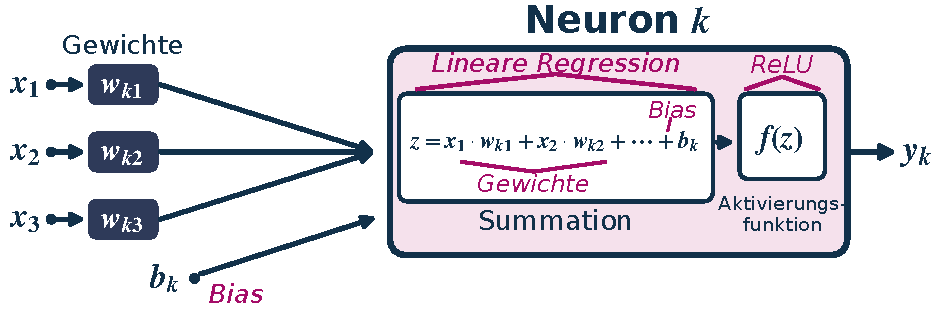
\includegraphics[width=0.8\columnwidth]{Images/neural-network-artificial-neuron-weights-bias-activation.pdf}
\end{center}
\end{contentbox}
\subsection{MLP (Standard Neural Network)}\label{sec:10-standard-neural-network-mlp}
\ZSFindex{Neuronales Netzwerk}
\ZSFindex[mlp]{MLP / Multilayer Perceptron}
\subsubsection{Neuron, Gewichte und Bias}
\begin{contentbox}
Ein \ZSFkeyword*{Neuron} berechnet:
\[
y_k = f(x_1 \cdot w_{k1} + x_2 \cdot w_{k2} + \cdots + x_n \cdot w_{kn} + b_k)
\]
\begin{factlist}
\ZSFFact{$x_i$}{Eingabewerte}
\ZSFFact{$w_{ki}$}{Gewichtung: Wie stark eine Eingabe zählt}
\ZSFFact{$b_k$}{Bias: verschiebt die Reaktionsschwelle}
\ZSFFact{$f$}{Aktivierungsfunktion: formt das berechnete Signal (siehe unten)}
\ZSFFact{Ablauf}{Gewichten $\to$ Bias addieren $\to$ Aktivierung anwenden}
\ZSFFact{Training}{Gewichtungen $w_{ki}$ und Bias $b_k$ werden im Training angepasst}
\end{factlist}
\end{contentbox}

\subsubsection{Aktivierungsfunktionen}
\ZSFindex{Aktivierungsfunktion}
\ZSFindex{ReLU}
\ZSFindex{Sigmoid}
\begin{contentbox}[ReLU und Sigmoid]
\begin{factlist}
\ZSFFact{ReLU}{Negative Werte $\to 0$, positive bleiben; oft in versteckten Schichten}
\ZSFFact{Sigmoid}{$\sigma(x) = \frac{1}{1 + e^{-x}}$ — Ausgabe bei binärer Klassifikation}
\end{factlist}
\end{contentbox}

\begin{statementbox}[Warum nichtlinear?]
Nur lineare Aktivierung ($f(x)=x$) lässt ein tiefes Netz zu einer einzigen linearen Schicht zusammenfallen. Erst Nichtlinearität (ReLU, Sigmoid) macht zusätzliche Schichten ausdrucksstark.
\end{statementbox}

\begin{contentbox}[Sigmoid: interner Wert $\to$ Wahrscheinlichkeit]
\begin{center}
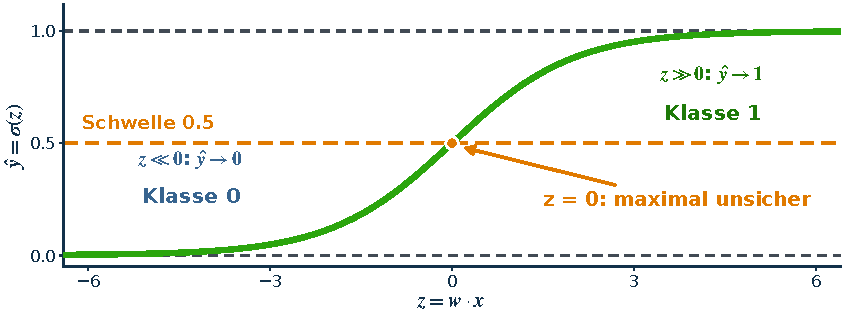
\includegraphics[width=0.72\columnwidth]{Images/neural-network-sigmoid-threshold-interpretation.pdf}
\end{center}
\end{contentbox}

\subsection{Softmax (Ausgabe für mehrere Klassen)}\label{sec:10-softmax-schicht-ausgabe}
\ZSFindex{Softmax}
\begin{contentbox}
\begin{factlist}
\ZSFFact{Idee}{Wandelt Ausgaben in Wahrscheinlichkeiten um:
    \[
    P_i = \frac{\exp(z_i)}{\sum_j \exp(z_j)} \quad \text{mit} \quad \sum_i P_i = 1
    \]}
\ZSFFact{Einsatz}{Wird bei Mehrklassenklassifikation als Ausgabeschicht genutzt}
\ZSFFact{Lesen}{Klassen konkurrieren; alle Wahrscheinlichkeiten zusammen $=1$.}
\end{factlist}
\end{contentbox}

\subsection{CNN (Convolutional Neural Network für Bilder)}\label{sec:10-convolutional-neural-network-cnn}
\ZSFindex[cnn]{CNN / Convolutional Neural Network}
\subsubsection{Convolution und Pooling}
\ZSFindex{Convolution}
\ZSFindex{Pooling}
\begin{contentbox}
Ein Neuron in einem Convolutional Neural Network (CNN) entsteht durch folgende Schritte:

\begin{factlist}
\ZSFFact{Convolutional Filter}{Kleiner Filter (z.\,B. $2 \times 2$) wird auf Bildbereiche angewendet.
Ergebnis wird durch eine Aktivierungsfunktion verarbeitet (z.\,B. ReLU)}
\ZSFFact{Pooling Layer}{Kleine Pooling-Matrix (z.\,B. $2 \times 2$) mit Aggregationsfunktion, typischerweise \ZSFkeyword*{MAX}}
\end{factlist}

\end{contentbox}

\begin{enumerate}[leftmargin=\ZSFprocLeftMargin,labelsep=\ZSFprocLabSep,itemsep=\ZSFprocItemSep,topsep=0pt,parsep=0pt,partopsep=0pt]
\ProcStep{Filter anwenden}{Anwenden des Filters auf die Eingabematrix}
\ProcStep{ReLU anwenden}{Anwenden der ReLU-Funktion auf jedes Element des Ergebnisses (setzt jeden negativen Wert auf 0)}
\ProcStep{Pooling}{Abschliessend: Anwenden der Pooling-Matrix (z.\,B. MaxPooling)}
\end{enumerate}

\begin{contentbox}[CNN: Convolution + Pooling]
\begin{center}
    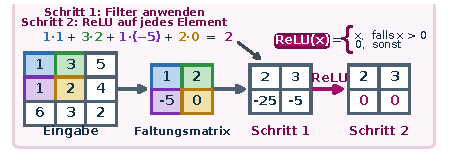
\includegraphics[width=0.8\columnwidth]{Images/cnn-convolution-filter-relu-steps.pdf}
\end{center}
\end{contentbox}

\subsection{Zusammenfassung}\label{sec:10-zusammenfassung}
\begin{contentbox}
\begin{factlist}
\ZSFFact{MLP}{Gut für strukturierte Daten (z.\,B. Tabellen) \ZSFsectionref{sec:10-standard-neural-network-mlp}}
\ZSFFact{CNN}{Gut für unstrukturierte Bilddaten \ZSFsectionref{sec:10-convolutional-neural-network-cnn}}
\ZSFFact{Versteckte Schichten}{meist ReLU}
\ZSFFact{Ausgabeschicht}{Sigmoid bei binärer Klassifikation; Softmax bei Mehrklassenklassifikation \ZSFsectionref{sec:10-softmax-schicht-ausgabe}}
\ZSFFact{Training}{Lernen erfolgt über Anpassung der Gewichtungen $w$ und Bias-Terme~$b$}
\end{factlist}
\end{contentbox}
